\documentclass[11pt]{article}
\usepackage{amsmath, amssymb}
\usepackage{geometry}
\geometry{margin=1in}
\usepackage{fancyhdr}
\usepackage{lastpage}
\usepackage{parskip} % Better paragraph spacing
\usepackage{titlesec} % Better section formatting
\usepackage{graphicx}
\usepackage{float}
\usepackage[most]{tcolorbox}
\usepackage{lmodern}
\usepackage{caption}

% Define commands for reusable content
\newcommand{\coursename}{CS-401 Applied Data Analysis}
\newcommand{\lecturenum}{06}
\newcommand{\lecturedate}{\today}
\newcommand{\professor}{Maria Brbic}

% Configure section spacing
\titlespacing*{\section}{0pt}{2ex plus 1ex minus .2ex}{1.5ex plus .2ex}
% Header / Footer
\pagestyle{fancy}
\fancyhf{}
\fancyhead[L]{\coursename}
\fancyhead[R]{Lecture \lecturenum}
\fancyfoot[L]{EPFL - Computer Science}
\fancyfoot[C]{Author: Jonathan Dutoit}
\fancyfoot[R]{Page \thepage\ of \pageref{LastPage}}

\begin{document}

\begin{center}
  {\large EPFL - Computer Science} \\[0.5em]
  {\Large \textbf{\coursename}} \\[0.5em]
  {\large Lecture \lecturenum\ --- \lecturedate} \\[0.5em]
  {\large Author: Jonathan Dutoit} \\[0.5em]
  {\large Professor: \professor} \\[0.5em]
\end{center}

\vspace{2cm}

\begin{center}
  {\LARGE \textbf{Causal analysis of observational data}}
\end{center}

\vspace{1cm}

\section*{Goal of this lecture}

\begin{itemize}
	\item Clarify difference between \textbf{experimental} and \textbf{observational} studies
	\item Highlight \textbf{pitfalls} of observational studies
	\item Give you \textbf{tools} for avoiding the pitfalls, allowing you to draw valid conclusions from "found data" (very useful for project!)
	\item Motivate you to \textbf{read} Rosenbaum's great book \href{http://www.stewartschultz.com/statistics/books/Design%20of%20observational%20studies.pdf}
	\item in particular Chapters 1, 2, and 3; 
\end{itemize}

\section*{Randomized controlled experiments}
\begin{itemize}
	\item Two experimental conditions:
		\begin{itemize}
			\item Treatment (e.g., medicine)
			\item Control (e.g., placebo)
		\end{itemize}
	\item Assignment of participants to conditions is random
		\begin{itemize}
			\item Probability of receiving treatment same for everyone
		\end{itemize}
	\item Treatment and control groups are indistinguishable
		\begin{itemize}
			\item E.g., determination to quit smoking is not systematically higher in the treated group
		\end{itemize}
\end{itemize}

\section*{Limits of randomization}

\begin{itemize}
	\item Do seat belts save lives?
	\item Experiment:
		\begin{itemize}
			\item Flip coin at birth to assign to treatment (always wear set belt for entire life) or control (never wear seat belt)
			\item Measure fraction of traffic deaths in each group
		\end{itemize}
	\item Randomized experiments aren't always feasible
		\begin{itemize}
			\item Unethical, expensive, fundamentally impossible (e.g., do earthquakes decrease life spans?)
			\item Most modern "big data" is "found data"
		\end{itemize}
	\item Experiments may lead to unrealistic scenarios	
\end{itemize}

\section*{Alternative: observational studies}
\begin{itemize}
	\item Fundamentally different from experiment:
		\begin{itemize}
			\item Researcher can't control who goes to which condition
			\item Researcher is merely an observer, not a tinkerer
			\item Much less problematic w.r.t. ethics, price, feasibility
			\item Much more problematic w.r.t. validity of conclusions
		\end{itemize}

	\item All advantages of randomized experiment are gone
		\begin{itemize}
			\item Subjects self-select to be treated
			\item Treatment assignment and response may be caused by same hidden correlate (a.k.a cofounders; e.g., motivation to quit smoking)
		\end{itemize}
\end{itemize}

\section*{Example: seat belts revisited}
\begin{itemize}
	\item Recall: experiment infeasible because unethical
	\item Observational study:
		\begin{itemize}
			\item Dataset: all traffic accidents in a given time span
			\item Two treatment conditions:
				\begin{itemize}
					\item Treated: seat-belt wearers
					\item Control: non-seat-belt wearers
				\end{itemize}
			\item Compare fraction dead in treated vs. control
		\end{itemize}
	\item What problems do you see? \\ 
	Maybe some people are more cautious driver (maybe because they are not using seat belt). Another, the position in the car may influence the likelihood of dying. Age could also be a factor, the car (old cars may not have airbags), etc...
\end{itemize}

\section*{As a causal diagram}

% Quick centered image
\begin{figure}[H]
    \centering
    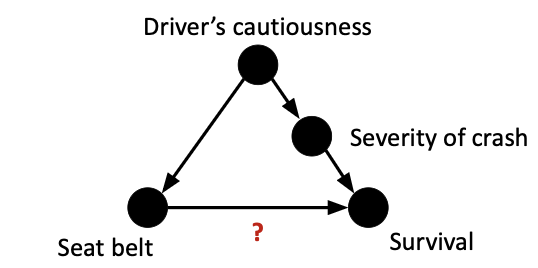
\includegraphics[width=0.6\textwidth]{causal}
    \label{fig:LABEL}
\end{figure}

\section*{A matched observational study}
\begin{itemize}
	\item Consider only a particular subset of accident cars:
		\begin{itemize}
			\item 2 people in car: driver + passenger
			\item Exactly one of them died in accident
			\item Exactly one of them wore seat belt at time of accident (i.e., 1 treated + 1 control per car)
		\end{itemize}

	\item As before: compare fraction dead in treated vs. control
	\item New: many potential co-founders are controlled for, including type of car, speed, severity of accident
	\item Fundamental concept: \textbf{\textcolor{purple}{matching}}
\end{itemize}

\section*{Setlling the seat-belt question}
% Quick centered image
\begin{figure}[H]
    \centering
    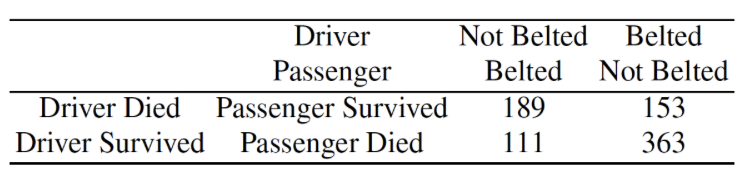
\includegraphics[width=0.7\textwidth]{seat-belt}
    \label{fig:LABEL}
\end{figure}

\section*{Natural experiments}

\begin{itemize}
	\item Not researches, but nature, "flips a coin" to decide treatment assignments
	\item Examples: twin studies
	\item Rosenbaum: "When investigators are especially proud, having found unusual circumstances in which treatment assignment, though not random, seems unusually haphazard, they may speak of a ‘natural experiment.”
	\item Is matched seat-belt study a natural experiment?
\end{itemize}

\section*{Nature didn't flip a coin for me -- should I go home and weep?}

\begin{itemize}
	\item No! You can still get good mileage if you're smart about it
	\item Fundamental concept: \textbf{\textcolor{purple}{matching}}
	\item Ideally: Pair up 2 identical people:
		\begin{itemize}
			\item 1 treated, 1 control
			\item Ex-post (vs. natural experiment: ex-ante)
		\end{itemize}
	\item Compare outcome of treated vs. control
	\begin{itemize}
		\item e.g, mean difference treated-minus-control
		\item or regression analysis 
	\end{itemize}	
	\item Such ideal matching usually not feasible
		\begin{itemize}
			\item \textcolor{red}{Problem 1:} \textbf{Unobserved covariates}: 
		\begin{itemize}
			\item You usually can't even know if two people are identical
			\item e.g., (hypothetical) gene that causes both desire to smoke and lung cancer
		\end{itemize}
			\item \textcolor{blue}{Problem 2:} \textbf{Combinatorial explosion}: \\
		(Nearly) no two people are identical
		\end{itemize}
\end{itemize}

\section*{Addressing Problem 1 by ignoring it: A naive model}

\begin{tcolorbox}[
  colback=yellow!15,     % background color
  colframe=black!50,    % border color
  boxrule=1pt,       % border thickness
  arc=3mm,             % rounded corners
  left=4mm, right=4mm, top=2mm, bottom=2mm % padding
]
"People who look comparable are comparable" \\

or equivalently: \\

"Only observed covariates determine treatment assignment"
\end{tcolorbox}
% Quick centered image
\begin{figure}[H]
    \centering
    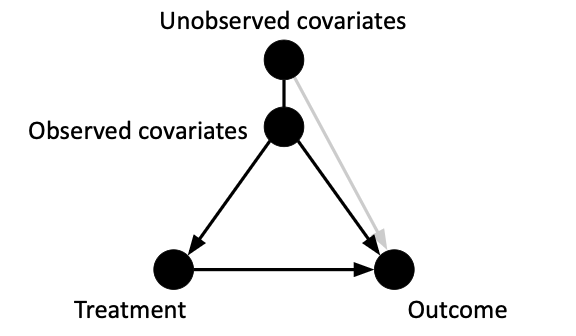
\includegraphics[width=0.5\textwidth]{naive}
    \label{fig:LABEL}
\end{figure}

Unobserved covariates can't affect the treatment! Furthermore, we don't care how observed and unobserved covariates are related.  

Example: 
\begin{itemize}
	\item Unobserved covariates: motivation to quit smoking
	\item Observed covariates: gender of people
\end{itemize}

\textbf{Note}: Some gender may have a higher motivation to quit smoking, but this doesn't affect the treatment directly! 

\textbf{\textcolor{red}{If the naive model was true...}}

\begin{itemize}
	\item ... you could "simulate" a randomized experiment:
		\begin{itemize}
			\item Simply match subjects with identical observed covariates (1 treated, 1 control) 
			\item Subjects in a pair have the same probability to treat 
			\item So who gets treated is up to chance, as in experiment
			\item Analysis: compare outcome for treated to outcome of control (e.g., mean difference treated-minus-control)
		\end{itemize}
\end{itemize}

\section*{Problem 2: Combinatorial explosion}

\begin{itemize}
	\item (Nearly) no two people are identical
	\item So finding two people to match is often impossible
		\begin{itemize}
			\item Even when considering only observed covariates (as in the naive model)
		\end{itemize}
	\item Do we really need to match people with identical \textbf{covariates}?
	\begin{itemize}
		\item Recall "holy grail": randomized controlled trials
		\item Coin makes sure everyone has identical \textbf{probability to be treated}
		\item  $\Rightarrow$ Let's mimic what the coin does!
	\end{itemize}
\end{itemize}

\section*{Addressing Problem 2: Propensity score}
\begin{itemize}
	\item Compress the (potentially many) observed covariates into a single number: the probability to receive the treatment (a.k.a. \textcolor{green}{propensity score}): 
		\begin{center}
			\verb|Pr(subject is treated| $|$ \verb|observed covariates)|
		\end{center}
	\item Can be estimated from the data
		\begin{itemize}
			\item E.g., via logistic regression
			\item Input: observed covariates
			\item Output: treatment indicator (1 if treated, 0 if control)
		\end{itemize}
\end{itemize}

% Quick centered image
\begin{figure}[H]
    \centering
    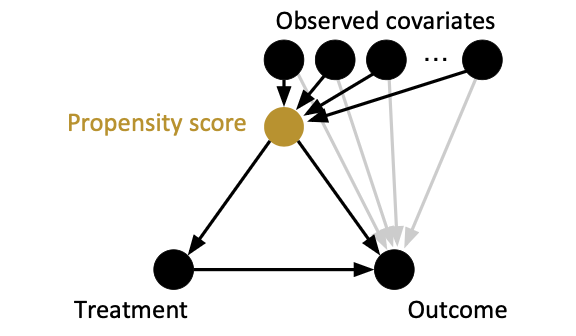
\includegraphics[width=0.6\textwidth]{propensity}
    \label{fig:LABEL}
\end{figure}

\section*{Balancing property of propensity score}
\begin{itemize}
	\item Fact: all subjects (treated and control) with equal propensity score (PS) \textit{p} have equal distribution of observed covariates \textbf{x}:
	\begin{center}
		Pr(\textbf{x} $|$  \textcolor{red}{treated = 1}, PS = \textit{p}) = Pr(\textbf{x} $|$  \textcolor{red}{treated = 0}, PS = \textit{p})
	\end{center}
	\item Subjects in a matched pair might not have equal \textbf{x}, but treated and control groups will have similar distributions of \textbf{x}
\end{itemize}

\section*{Balancing property is propensity score's reason to be}
\begin{itemize}
	\item There are many other methods for achieving balance
		\begin{itemize}
			\item e.g., exact matching, Mahalanobis distance matchings, coarsened exact matching...
		\end{itemize}
	\item You can mix and match methods (e.g., match exactly on gender, use propensity score for other covariates)
	\item What eventually matters is whether you achieve balance
		\begin{itemize}
			\item Regardless of \textit{how you try to achieve balance}, you need to verify \textit{that you managed to achieve balance}
		\end{itemize}
\end{itemize}

% Quick centered image
\begin{figure}[H]
    \centering
    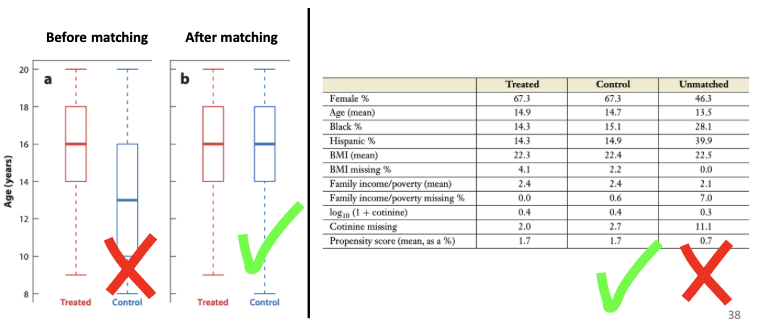
\includegraphics[width=1\textwidth]{balance}
    \label{fig:LABEL}
\end{figure}

\section*{Matching algorithms}

\begin{itemize}
	\item Goal: Match subjects into pair (1 treated, 1 control), with identical propensity scores within each pair
	\item Unlikely that 2 subjects have identical propensity scores
	\item Use approximate matching (remember your algo class!)
	\item Bipartite graph: each subject connected to all other subjects 
	\item Edge weights: absolute (or squared) difference of propensity scores (or other matching criterion)
	\item Find minimum matching, e.g., via Hungarian algorithm
\end{itemize}

% Quick centered image
\begin{figure}[H]
    \centering
    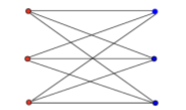
\includegraphics[width=0.3\textwidth]{bipartite}
    \label{fig:LABEL}
\end{figure}

\textbf{\textcolor{red}{If the naive model isn't true...}}

\begin{itemize}
	\item ... propensity score may differ from true probability to treat:
		\begin{center}
			Pr(treated $|$ observed covariates)  $\neq$ Pr(treated  $|$ all covariates)
		\end{center}
\end{itemize}

% Quick centered image
\begin{figure}[H]
    \centering
    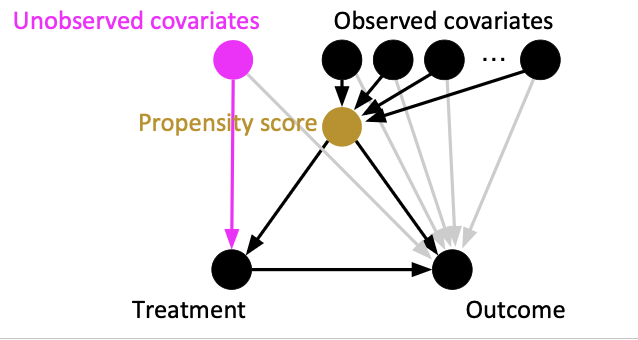
\includegraphics[width=0.6\textwidth]{violated-naive}
    \label{fig:LABEL}
\end{figure}


\textbf{\textcolor{red}{If the naive model isn't true}}, you may end up matching 2 peoples that are different but have similar description...

% Quick centered image
\begin{figure}[H]
    \centering
    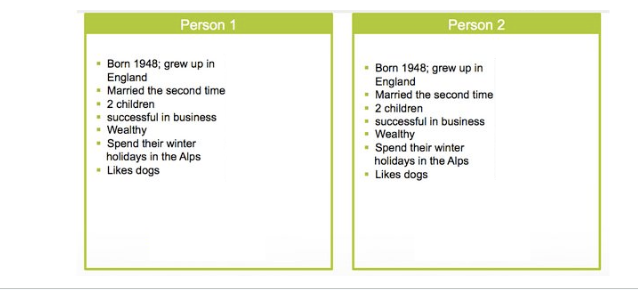
\includegraphics[width=0.9\textwidth]{person}
    \label{fig:LABEL}
\end{figure}

\section*{The sensitivity analysis model}

\begin{itemize}
	\item \textbf{Idea}: Quantify the degree to which the naive model may be wrong without you having to change your (casual) conclusions
	\item Assume that treatment odds of identical-looking-subjects (i.e., identical observed covariates \textbf{x}) \textcolor{purple}{may differ by up to a factor $\Gamma$}
	\item Then reason in spirit of proof by contradiction: "To change the conclusions of my study, two identical-looking people (1 treated, 1 control) would have to have hugely different treatment odds (i.e., huge $\Gamma$). Common sense (or domain knowledge) suggests that this is no the case, so my conclusions stand".
\end{itemize}

\[
	\frac{1}{\Gamma} \leq \frac{\pi_k / (1 - \pi_k)}{\pi_l / (1 - \pi_l)} \leq \Gamma \text{    whenever \textbf{x}$_k$ = \textbf{x}$_l$. $\Gamma \geq 1$}
.\] 

\begin{itemize}
	\item Bounded odds ratio (OR)
		\begin{itemize}
			\item Reason for using OR: \\
			OR = Pr(\textit{k} treated $|$ \textbf{either \textit{k} or \textit{l} treated}) / Pr(\textit{l} treated $|$  \textbf{either \textit{k} or \textit{l} treated})
		\end{itemize}
	\item Sensitivity $\Gamma = 1 \Rightarrow$ naive model is true  
	\item Sensitivity $\Gamma = 2 \Rightarrow$ subject with same observed covariates \textbf{x} up to twice as likely to be the one to receive treatment 
	\item Sensitivity $\Gamma = \infty \Rightarrow$ avoid statement (a.k.a. tautology) 
\end{itemize}

\section*{Example: smoking and lung cancer}

\begin{itemize}
	\item \textcolor{purple}{Under naive model}: matching on observed covariates gives a very small \textit{p}-value for the null hypothesis that smoking does not increase lung cancer risk (using appropriate hypothesis test), i.e., data hard to explain without a causal effect
	\item \textcolor{green}{Tobacco lobby:} "The naive model isn't true! There may be a hidden (e.g., genetic) correlates that increase both the probability to enjoy smoking and the probability of lung cancer. They, not smoking, cause cancer!
	\item Under sensitivity analysis model, increasing sensitivity $\Gamma$ increase the  \textit{p}-value for null hypothesis
	\item \textcolor{purple}{Anti-tobacco lobby}: "But making \textit{p} $>$ 0.05 would require  $\Gamma >$ 6; i.e., the odds of being a smoker would need to be six times higher for one of two people with the exact same observed features (age, gender, education, income, ...). It's unlikely that any unobserved covariate would have such a large effect on smoking habits. So smoking causes cancer!"
\end{itemize}


\section*{Two parts: mechanical vs. scientific}
\begin{itemize}
	\item Mechanical part:
		\begin{itemize}
			\item Create pairs (1 treated + 1 control) with similar observed covariates (using exact or propensity-score matching)
		\end{itemize}
	\item Scientific (i.e., fun) part:
		\begin{itemize}
			\item Mitigate concerns that your findings might be caused by unobserved covariates, rather than treatment (e.g., using sensitivity analysis, ad-hoc arguments, natural experiments)
		\end{itemize}
\end{itemize}

\section*{Summary}
\begin{itemize}
	\item Holy grail: \textcolor{orange}{randomized experiment}
	\item When experiment not possible: \textcolor{purple}{observational study}
	\item Crucial problem: treatment assignment not random (biases!)
	\item Semi-holy grail: \textcolor{green}{natural experiment}
	\item \textcolor{blue}{Matches studies}: pair up treated/control based on observed covariates
	\item Problem: still, treatment assignment not random (biases via unobserved covariates)
	\item Solution: \textcolor{red}{sensitivity analysis}
	\item Keep this lecture in mind for your projects!
\end{itemize}



\end{document}
